\documentclass{article}

\usepackage{color}
\usepackage{epsfig,graphics}
\usepackage{amsmath}

\usepackage[utf8]{inputenc}
\usepackage[protrusion=true,
            expansion=true
           ]{microtype}

\usepackage[slovene]{babel}
\usepackage{graphicx} 
\usepackage{caption}          % Needed for including graphics.
\usepackage{url}                % Facility for activating URLs.

\usepackage[a4paper,margin=2.4cm]{geometry}

\usepackage{tikz}
\usetikzlibrary{shapes.geometric, arrows}
\tikzstyle{input} = [trapezium, trapezium left angle=70, trapezium right angle=110, minimum width=3cm, minimum height=1cm, text centered, draw=black, fill=blue!30]
\tikzstyle{startstop} = [rectangle, rounded corners, minimum width=3cm, minimum height=1cm,text centered, draw=black, fill=red!30]
\tikzstyle{process} = [rectangle, minimum width=3cm, minimum height=1cm, text centered, text width=7cm, draw=black, fill=orange!30]
\tikzstyle{decision} = [diamond,aspect=2, minimum width=3cm, minimum height=1cm, text centered, draw=black, fill=green!30]
\tikzstyle{arrow} = [thick,->,>=stealth]

\begin{document}
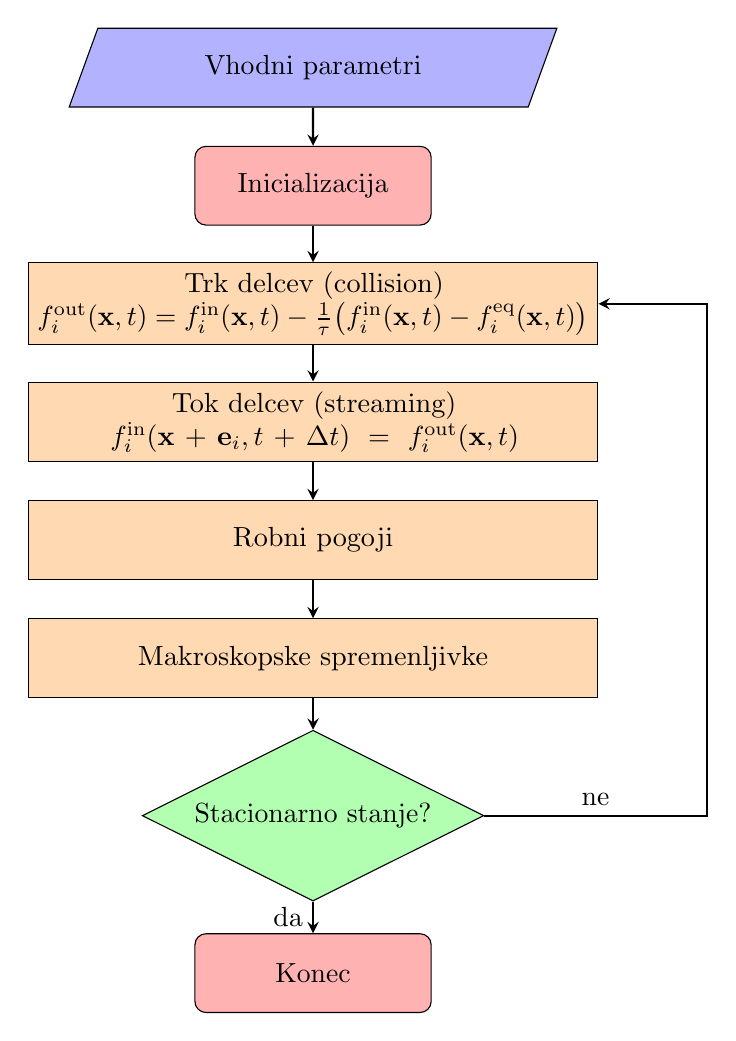
\begin{tikzpicture}[node distance=1.5cm]

\node (vhod) [input] {Vhodni parametri};
\node (start)[startstop, below of=vhod] {Inicializacija};
\node (pro1) [process, below of=start] {Trk delcev (collision)\\
$f^{\mathrm{out}}_i(\mathrm{\mathbf{x}},t)=f^{\mathrm{in}}_i(\mathrm{\mathbf{x}},t)-\frac{1}{\tau}\big(f^{\mathrm{in}}_i(\mathrm{\mathbf{x}},t)-f^{\mathrm{eq}}_i(\mathrm{\mathbf{x}},t)\big)$};
\node (pro2) [process, below of=pro1] {Tok delcev (streaming)\\
$f^{\mathrm{in}}_i(\mathrm{\mathbf{x}}+\mathrm{\mathbf{e}}_i,t+\Delta t)=f^{\mathrm{out}}_i(\mathrm{\mathbf{x}},t)$};
\node (pro3) [process, below of=pro2] {Robni pogoji};
\node (pro4) [process, below of=pro3] {Makroskopske spremenljivke};
\node (dec1) [decision, below of=pro4, yshift=-0.5cm] {Stacionarno stanje?};
\node (stop) [startstop, below of=dec1, yshift=-0.5cm] {Konec};


\draw [arrow] (vhod) -- (start);
\draw [arrow] (start) -- (pro1);
\draw [arrow] (pro1) -- (pro2);
\draw [arrow] (pro2) -- (pro3);
\draw [arrow] (pro3) -- (pro4);
\draw [arrow] (pro4) -- (dec1);
\draw [arrow] (dec1) -- node[anchor=south] {ne} ++(5,0) |- (pro1);
\draw [arrow] (dec1) -- node[anchor=east] {da} (stop);

\end{tikzpicture}
\end{document}
